\subsection{Training Maps}
\label{sec:navtasks}
We evaluate the Nav-A3C algorithm on maps with 5 stages of difficulty. While the Nav-A3C algorithm works smoothly on the first four stages, it does not perform better than bug-exploration methods on the 5th stage.
We propose these experiments as a 5-stage benchmark for all end-to-end navigation algorithms.

%While there already exists optimal algorithms to find shortest path between two points and perform optimal navigation between given set of points in a given map, the advantage of Deep reinforcement learning comes from its ability to extract required features from the input images and its promise
%optimize mapping and path planning in end-to-end fashion. 
%Thus we need to either integrate existing path planning and mapping methods with deep learning methods to perform end-to-end training or extend deep learning methods to learn path planning and mapping.

\begin{description}
  \ditem{Static goal, static spawn and static map}
  \label{prob:sss}
   This is the easiest variation of our experiments with the environment
   being completely deterministic. 
   To perform optimally on this experiment, the agent needs to find and learn the
   shortest path at trainng time and repeat it during testing. 
  \ditem{Static goal, random spawn and static map}
  This is a textbook version of the reinforcement learning problem, especially in gridworld \cite{SuBaBOOK1998}, with the only different being that the environment partially instead of fully observable.
  This problem is more difficult than Problem~\ref{prob:sss} because the agent
  must find an optimal policy to the goal from each possible starting point in the maze.
  \ditem{Random goal, static spawn and static map}
  This experiments highlights the map-exploitation ability of the agent. To perform well, the agent must remember and exploit a goal location after it has been discovered so that it may continue to revisit it.  
  
  Following \cite{MiPaViICLR2017}, we report the ratio
  of time taken to hit the goal for the first time (exploration time) vs the average amount of time taken to hit goal subsequently (exploitation time). The metric, called \LatencyOneGtOne{}, is a measure of the map-exploitation ability of the agent. 
  If this ratio is greater than 1, then we say that the agent is doing better than random exploration.
  \ditem{Random goal, random spawn and static map}
  In this version of the experiment both the spawn point and the goal location is randomized. To perform optimally, the agent must localize itself within the map in addition to being able to exploit map-information.
  
  This is the problem that is addressed by \cite{MiPaViICLR2017} with limited success. 
  They evaluate this case on two maps and report \LatencyOneGtOne{} to be greater than 1 in one of the two maps. We evaluate the same metric on ten other maps and provide the tools for application to several more.
  \ditem{Random goal, random spawn and random map}
    We believe that any proposed algorithms on end-to-end navigation problems, should be evaluated on unseen maps.
    To our knowledge, this is the first paper to do so in the case of deep reinforcement learning based navigation methods.
    We train agents to simultaneously learn to explore 1, 10, 100, 500 and 1000 maps and test them on the same 100 unseen maps. The relevant reward curves showing performance over training and testing can be found in Fig~\ref{fig:plot_reward_on_testing}. 
\end{description}

The comparitive evaluation of different the stages of this benchmark are shown in Fig~\ref{fig:latency-goal-reward}.

\subsection{Evaluation Maps}
We also evaluate the algorithm on a few qualitative maps other than I-maze. These maps are specifically designed to query what percentage of times does the agent takes shortest path.

\setcounter{Benchmark}{0}
\begin{description}
    \ditem{Wrench map}
    This map is shown on the top row, extreme right column in Fig~\ref{fig:environments}. It has one loop and a corridor.
    The goal is placed asymmetrically in the loop and the agent is spawned in the corridor.
    Because of asymmetrical placement of the goal, one of the path to the goal is shorter than the other and there are only two possible paths.
    We record the path taken each time. If the agent has learned a greedy strategy, then it would repeat the path taken for the first time.
    We evaluate the fraction of times, the agent repeats the first path. A higher number indicates a greedy strategy.
    In second evaluation, we let the agent explore randomly untill it hits the goal via the shorterst path.
    At this point we evaluate the  fraction of times shortest path is taken. For this score 
    \ditem{Goal map}
    This map is shown on the bottom row, extreme right column in Fig~\ref{fig:environments}.
    We chose this map because this is the simplest map with a fork. Making the map any simpler will make the map homeomorphic to a straight line. 
    We evaluate the number of times the agent takes the right descision at the fork after exploring the goal once.
\end{description}

\begin{figure}%
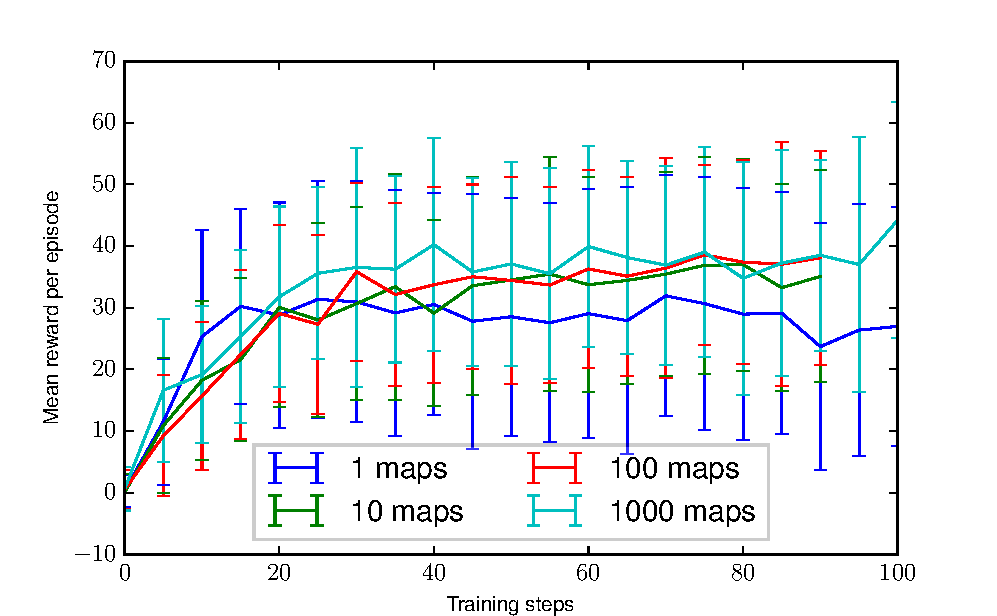
\includegraphics[width=0.5\columnwidth]{images/plot_reward_3D-1000.pdf}%
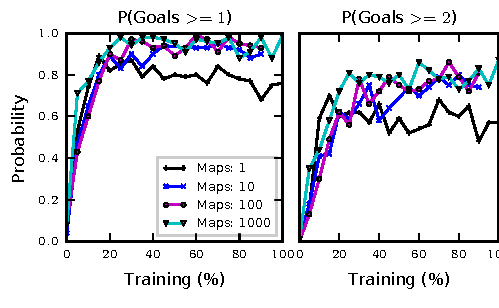
\includegraphics[width=0.5\columnwidth]{images/plot_probability_3D-1000.pdf}%
\vspace{-1em}%
\caption{Mean reward while tested on 100 unseen maps, while being trained on different number of training maps. Note that while training on 1000 maps eventually achieves high reward, it is only higher mean reward (44.2), training on 1 map hits the maximum (31) much faster.}%
\label{fig:plot_reward_on_testing}%
\end{figure}
